\subsection{Conditional Branching with Statement Nodes}

{\bf \large this is appendix content. Be sure to review to make sure it flows with the document. Is it only Visual?}

When working with SDMs, you often need to choose between two different patterns based on the return value of an arbitrary (black box) operation.
This is like the normal \texttt{Success}/\texttt{Failure} construction, but instead of a pattern being matched or failing, the decision can be implemented with
a another SDM or a standard Java method. This feature is a further means (besides \texttt{MethodCallExpressions} for attribute values and \texttt{Bindings}) of
integrating hand-written Java code in SDMs (and can lead to spaghetti SDMs so please use with caution!).

As an example, consider a class \texttt{A} with an operation:
\begin{quote}
 \mbox{\texttt{doSomeCheck(p$_1$,\ldots,p$_n$ :EClass) :EBoolean}}
\end{quote}

This method could be implemented in hand-written Java code or be specified by another SDM specification.

Although dummy boolean attributes \emph{could} be used to achieve the same effect, it is much simpler to branch the control flow based on the result of a \texttt{StatementNode}.
If the method returns an \texttt{EBoolean}, \texttt{Success} and \texttt{Failure} correspond to \texttt{true} and \texttt{false}, respectively. If the method returns anything else, then \texttt{Failure} corresponds to \texttt{null}. Void methods \emph{cannot} be used to branch and an exception is thrown during code generation.

Fig.~\ref{fig:cond_branch_on_op} depicts the class \texttt{A} and shows how \texttt{doSomeCheck} is used to branch in an SDM.
Fig.~\ref{fig:cond_branch_on_op_code} depicts the corresponding generated if/else branch in Java.

\begin{figure}[htp]
\begin{center}
  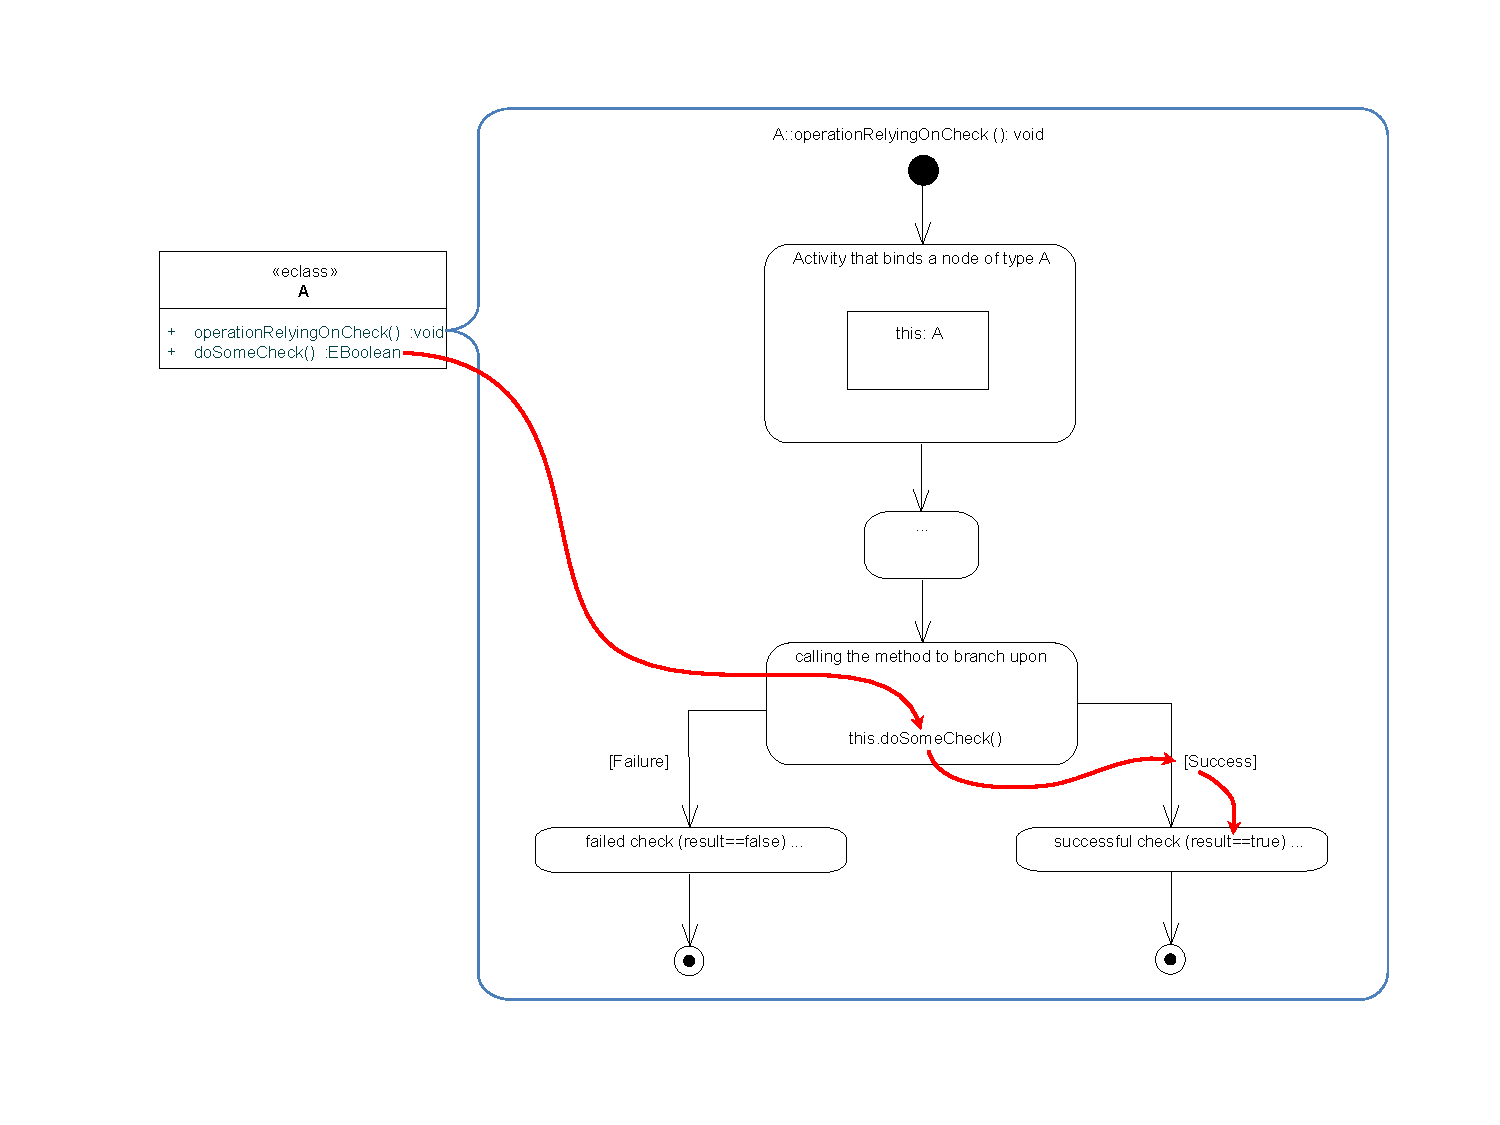
\includegraphics[width=1\textwidth]{SDM_with_branch}
  \caption{Conditional branching based on the result of an operation}
  \label{fig:cond_branch_on_op}
\end{center}
\end{figure}

\begin{figure}[htp]
\begin{center}
  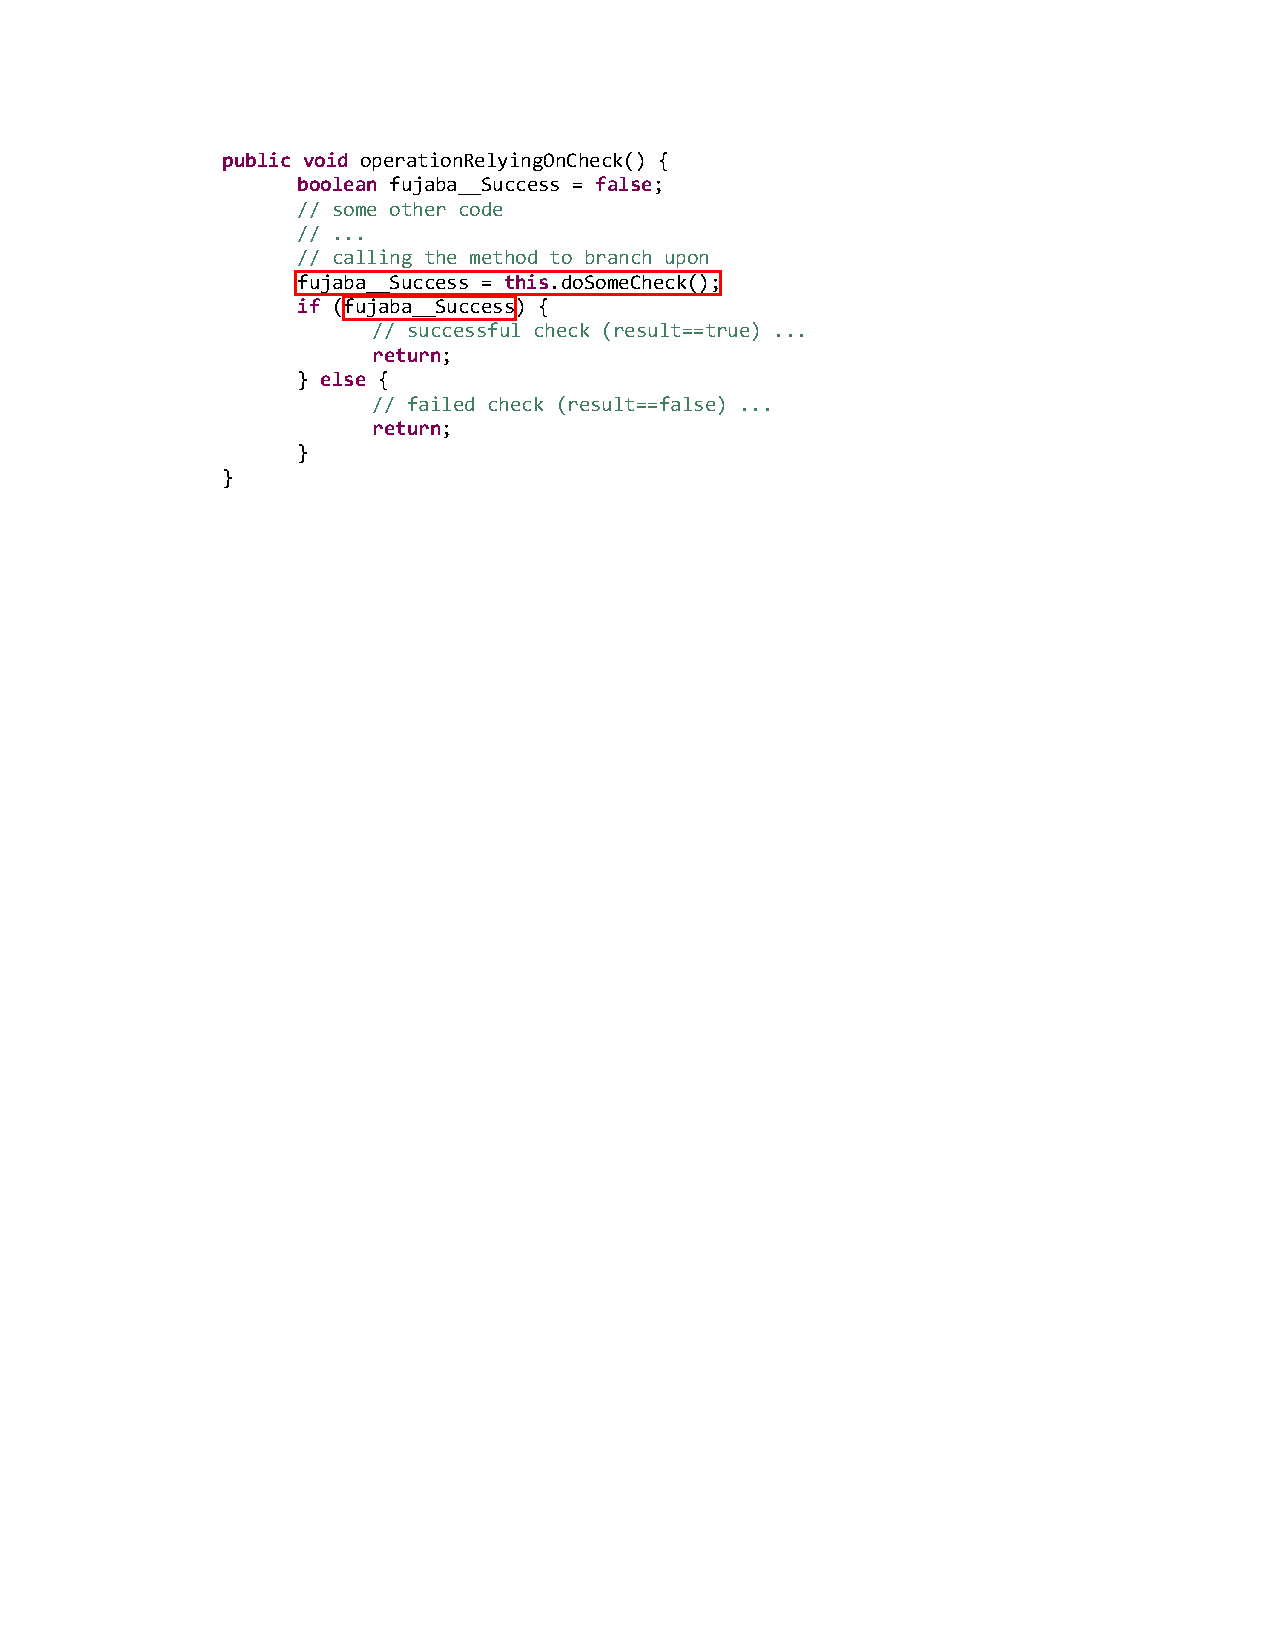
\includegraphics[width=0.7\textwidth]{generated_code}
  \caption{Generated code for branch}
  \label{fig:cond_branch_on_op_code}
\end{center}
\end{figure}

Perform the following steps to branch with a \texttt{StatementNode}:
\begin{enumerate}
\item[$\blacktriangleright$] Add a new statement node (cf.~Fig.~\ref{fig:cond_statement_node}) at the appropriate location in your SDM.
\item[$\blacktriangleright$] Invoke a non-void method (an operation in the metamodel) via a \texttt{MethodCallExpression} (cf.~Fig.~\ref{fig:cond_method_call}).
\item[$\blacktriangleright$] Add \texttt{Success} \emph{and} \texttt{Failure} edges to the \texttt{StatementNode} to branch appropriately.
\end{enumerate}

\begin{figure}[htp]
\begin{center}
  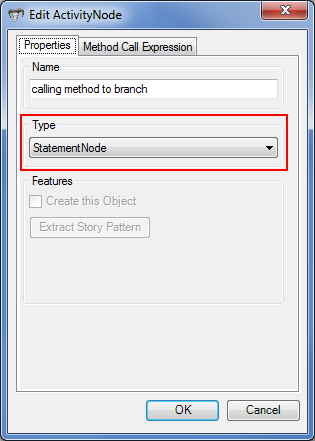
\includegraphics[width=0.5\textwidth]{01_switch_to_statement_node}
  \caption{Switch from activity node to statement node}
  \label{fig:cond_statement_node}
\end{center}
\end{figure}

\begin{figure}[htp]
\begin{center}
  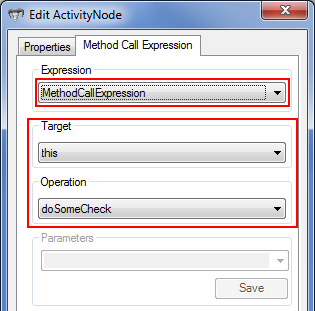
\includegraphics[width=0.5\textwidth]{02_specify_method_call_expression}
  \caption{Specify the method call expression}
  \label{fig:cond_method_call}
\end{center}
\end{figure}

\clearpage